\documentclass{acmsig}

\usepackage[color=yellow,obeyFinal]{todonotes}
\usepackage{graphicx}
\graphicspath{ {notebook/} }
\usepackage{epstopdf}
\usepackage{float}
\usepackage{varioref}
\usepackage{mathtools}
\usepackage{xspace}
\usepackage{subfigure}
\usepackage{hyperref}
\usepackage{balance}
\usepackage{listings}
\usepackage{algorithm}
\usepackage{algpseudocode}
\usepackage{paralist}
\usepackage{cite}
\usepackage{color}

\usepackage{xcolor}
\definecolor{dark-red}{rgb}{0.4,0.15,0.15}
\definecolor{dark-blue}{rgb}{0.15,0.15,0.4}
\definecolor{medium-blue}{rgb}{0,0,0.5}
\hypersetup{
  colorlinks, linkcolor={dark-red},
  citecolor={dark-blue}, urlcolor={medium-blue}
}

\newcommand{\etal}{\textit{et al.}\xspace}
\newcommand{\eg}{\textit{e.g.}\xspace}
\newcommand{\ie}{\textit{i.e.}\xspace}
\newcommand{\etc}{\textit{etc.}\xspace}
\newcommand{\vs}{\textit{vs.}\xspace}
\newcommand{\keyval}{$\langle\text{key}, \text{value}\rangle$\xspace}
\DeclarePairedDelimiter\floor{\lfloor}{\rfloor}


\newcommand{\noteby}[2]{\todo[inline]{#2\hspace*{\fill}\mbox{ --#1}}}

\lstset{frame=tb,
  language=SQL,
  aboveskip=3mm,
  belowskip=3mm,
  showstringspaces=false,
  columns=flexible,
  basicstyle={\small\ttfamily},
  numbers=none,
  numberstyle=\tiny\color{blue},
  stringstyle=\color{mauve},
  keywordstyle=\color{blue},
  commentstyle=\color{Brown},
  stringstyle=\color{mauve},
  breaklines=true,
  breakatwhitespace=true
  tabsize=3
}

% correct bad hyphenation here
\hyphenation{op-tical net-works semi-conduc-tor}


\begin{document}

% paper title
% can use linebreaks \\ within to get better formatting as desired
\title{The Impacts of Virtualization\\ on Big Data Application's Workload}


% author names and affiliations
% use a multiple column layout for up to three different
% affiliations
\numberofauthors{4}
\author{
\alignauthor
Ha Son Hai\\
       \affaddr{Orange/EURECOM}\\
       \email{sonhai@eurecom.fr}
\alignauthor
Daniele Venzano\\
       \affaddr{EURECOM}\\
       \email{venzano@eurecom.fr}
\and
\alignauthor
Patrick Brown\\
       \affaddr{Orange}\\
       \email{p.brown@orange.fr}
\alignauthor
Pietro Michiardi
       \affaddr{EURECOM}\\
       \email{michiard@eurecom.fr}
}

% make the title area
\maketitle


\begin{abstract}
Still very abstract
\end{abstract}

%%%%%%%%%%%%%%%%%%%%%%%%%%%%%%%%%%%%%%%%%%%%%%%%%%%%%%%%%%%%%%%%%%%%%
\section{Introduction}
%%%%%%%%%%%%%%%%%%%%%%%%%%%%%%%%%%%%%%%%%%%%%%%%%%%%%%%%%%%%%%%%%%%%%

The adoption of virtualization brings many benefits to the technology community. It gives ways to high flexibility, high availability and high utilisation of the hardware. But it also brings the disadvantages by adding complexity to the management and overhead to the performance. On the other hand, in 2014, IDG [1] published a study in which they found that more than 70\% of enterprise organizations have either deployed or are planning to deploy big data-related projects and programs [2]. Bringing big data application to the cloud is surely unavoidable in the future. We are seeing more and more Hadoop [3] or Spark [4] cluster operating on the cloud. The marriage of big data application and virtualization is already happened and continued to grow more and more greatly than ever. However, when mentioning about the performance of Big Data application on the cloud, people just walk away with the common thought that virtualization bringing bad performance to big data application because of the added virtualization layer. Yet we wonder, if it is really bad, how bad it is? to the most of our knowledge, there is no or very few works that directly studies the impacts of virtualization on the big data application performance.

\begin{figure}[htbp]
    \centering
    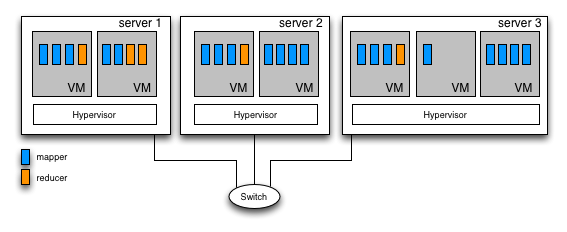
\includegraphics[width=0.5\textwidth]{figures/cluster_snapshot.png}
    \caption{\textit{An example snapshot of a running virtualised MapReduce cluster}}
    \label{cluster_snapshot}
\end{figure}

Measuring the performance of a distributed application is hard, and it is even harder when that application is running on virtualized platform which involving layers and layers of different technologies. Yet the measurement is necessary to have a proper understanding on performance of Big Data applications in the virtualized environment. Figure 1 is an abstract snapshot of a small MapReduce cluster operating in virtualized environment at a random time. There are 3 physical servers which host 7 Virtual Machines. These VMs were set-up as a Hadoop cluster and are running a Map Reduce job. To execute the job, the application initiates several parallel mappers and reducers inside each VM. Those threads are concurrently competing for the same resources at each physical host such as disk storage, memory, and CPU,... to perform their tasks. When looking at the whole picture, we see that the performance of the whole cluster is depended on the performance of every one of its building block: a physical host. To simplify the study, we select a physical host to be the foundation for the study and we model two basic and distinguished scenarios that can be seen on a physical host of a virtualized Hadoop cluster:
\begin{itemize}
\item Single VM with multiple threads (SVM-MT): this scenario (figure [?]) represents the case that the host has only one VM but this VM runs many mappers and reducers at the same time. This scenario is not rare to see because many administrators like to use fat VM for their cluster and the host can only host one fat VM. We consider 5 different flavors of VM for this scenario to see how the VM's size affects on the performance.
\item Multiple VMs with single thread (MVM-ST): this scenario (figure [?]) represents the case that we have a small VM and this VM runs only one mapper or reducer at a time. But because this is a virtualized environment and hardware resources are sharing between different customers, so there are many small VMs running on the same host. Those VMs do not know that they are competing for the same resources. This scenario is also not rare to see because the cloud administrators often share same servers for their different customers. Sharing physical resources is one of the reason that virtualization is adopted widely.
\end{itemize}
In reality, we have different mixes between the scenarios. However, we select those two since it focuses on different components of the same platform. The SVM-MT scenario focuses on the guest OS scheduler since it has to switch between active threads. The MVM-ST one focuses on the hypervisor scheduler since it has to switch between active VMs. Last but not least, the bare-metal system is used as the baseline to make the comparison (figure [?]). In case the big data application runs on a bare-metal environment, many mappers or reducers running at the same time requesting for IO resource. In short, it is similar to the case of SVM-MT but without virtualization. In this paper, we establish our focus only on the storage I/O performance since it was thought to be one of the main bottle necks of big data application [5]. More specific, we are especially interesting in the case that we have only one local hard drive on the server since there are often cases that data were stored on same disk or VM is running on same disk.

We consider I/O throughput and I/O fairness as the metrics to compare the performance between bare-metal and virtualized platform. The throughput metric expresses how well the system feed data to the threads while fairness keep threads away from data starvation. If one mapper cannot read data, it becomes stragglers and heighten End-Job Time which in the end reduce the responsiveness of the application. We also consider CPU utilization and the number of context switching in the experiment in order to understand the throughput result that we got. Before the study, our expectation was set on the conclusion of the overhead of virtualization on big data application workload. One part of our study repeats the findings of previous studies which show that virtualization can only reach 80-90\% of bare metal performance due to the overhead that the added virtualization layer brought up. However, that is only haft of the truth. Previous studies reveal the performance of the system when there is only one active thread that request for I/O. Our studies reveal the big picture when there are many active threads concurrently compete for I/O. And the discrepancy between scenarios only starts to show when there are more than 4 active threads/VMs requesting for IO resources. We see different performance between VM flavors. Fatter VM does not always mean better throughput. Our fattest VM gets only 60\% the throughput that a smaller one can get. We also see that bare-metal platform has problem when dealing with high level of concurrency. In our experiment, bare-metal platform can only achieve 25\% throughput in compare to a VM with 4 virtual cores. On the fairness of the systems, we see that both virtualized and bare-metal platform achieve very high fairness index. There is no different between bare-metal and virtualized platform in fairness.

We believe that the result from this work can help the communities to have more confident to deploy Big Data application on the cloud. However, this is just the first part in a continuation research which studies on the impacts of virtualization on Data Intensive Analysis Framework in which there are two most popular representatives: Hadoop and Spark. Hadoop and Spark performance can be bounded by network, disk I/O, or CPU performance. In this paper, we focus on disk I/O and it is the limitation of our work. Performance of Big Data application is not only depended on storage I/O performance, so when we view the performance from the application layer with actual big data workload, the result can be different or even opposite. In the next sections, we introduce to our readers our methodologies in detail. We also present the findings and explanation for the result that we got. Finally, we summarize our work at the last section and suggest the future approaches to give more meaningful results to the study.

%Guide from P.Pietro: Even we looking at the application level. Measure the impact of virtualization on the big data technology. we still need a proper understanding on what happens without the application because the application is very complex. it's a large distributed system that hides a lot of details so whenever you see the result, the problem is that it's very hard to explain what happened if you only look from the perspective of Hadoop or Spark. That was the reason why we simplify the thing. Let try to somehow emulate  what is the traditional workload generated by application such as Hadoop MapReduce. The question was what happens when you have the virtualization layer that hide in the middle between your application and IO call. And that why we have the measurement of bare-metal with several different configuration of the hard drive setting and CPU setting. We show that more or less the performance did not change much. So bare metal is really stable. And then we have result that look at different flavors of CPU of virtual machine with different size. And also the number of concurrent threads. These are the useful foundation for understanding the next result that you will obtain by running some sample of map reduce application which have similar workload. State what your goal are. You establish a measurement methodology where you explain your experimental setup, your tools, metrics, why they're important. And there you explain the statistical perspective of experiments. Then to validate your initial claim once the paper is done in the introduction (for example "we see that Hadoop on virtualization is suck"). You anticipate the result.

%to cite
%[1] http://www.idgenterprise.com/report/big-data-2

%%%%%%%%%%%%%%%%%%%%%%%%%%%%%%%%%%%%%%%%%%%%%%%%%%%%%%%%%%%%%%%%%%%%%
\section{Background and Related Work}
%%%%%%%%%%%%%%%%%%%%%%%%%%%%%%%%%%%%%%%%%%%%%%%%%%%%%%%%%%%%%%%%%%%%%
\begin{itemize}
  \item introduce some related works on the performance of virtualization: explaining packet delay under virtualization, works from Guillaume and Dino, work from IBM on performance of KVM, work from a guy discussing the relevant of IO schedulers to virtualization system.
  \item introduce some related works on measuring performance of data intensive application
 \item then mention about the combined of both, what we are different from previous works, what are our interesting points.
\end{itemize}
%%%%%%%%%%%%%%%%%%%%%%%%%%%%%%%%%%%%%%%%%%%%%%%%%%%%%%%%%%%%%%%%%%%%%
\section{Problem statement}

In the Big Data world, data volume is too big that people avoiding moving it. With the belief that network is the bottleneck of the distributed systems, the developers try to work around by moving the execution/programs to the workers but not the data (like Hadoop with MapReduce framework). By such way of task distributing, storage I/O (disk and memory) was fully utilised to get the most out of the data processing system. Hadoop reported 
One of the example is Spark, when they leverage memory to use together with the disk, Spark reported the performance improvement up to severalfold. However, memory and cache sharing was not developed well enough to provide fault tolerant to the distributed system. That is why the data intensive applications greatly depend on the hard drive performance.

In addition, the trending now is moving to the cloud, where people can rent a part of the virtualized infrastructure to process their data.
All of these brings the virtualization technology on top of choices to deploy data intensive application.

When running Hadoop/data intensive application in virtualized environment, the performance of the I/O now is very important. Everything depends on disk I/O. Data was read from disk, intermediate data was stored on disk, and results was written to disk. But the number of study (on this) are counting with just fingers.

There is a common belief that virtualization
We wonder if it is really true. And if it is bad, how bad it is? Is there any methodology that can help us to gain more performance with virtualization? In this report we present our study on the performance of I/O operation in virtualized environment. We make the experiments with the three layers: bare-metal (or the performance of host), guest operating system (or the performance of the VM), and application.



% cite: Locality-Aware Reduce Task Scheduling for MapReduce - Mohammed Hammoud, CloudCom
% cite: Purlieus: Locality-aware Resource Allocation for MapReduce in a Cloud - Balaji Balanisamy
% cite: Locality-Aware Dynamic VM Reconfiguration on MapReduce Clouds - Jongse Park

\begin{itemize}
  \item \textit{What we do?}
  \begin{itemize}
    \item Experimental study of virtualization overheads for I/O operations
    \item We want to have the typical I/O ``pressure'' that comes from data-intensive applications
    \item We want to have the view from the ``guest operating system'' and the view from the applications (and see if there are differences)
  \end{itemize}
  \item \textit{Why and why is it important?}
  \begin{itemize}
    \item It is common wisdom that virtualization is ``bad'' for performance. Is it true?
    \item Given the knowledge about performance bottlenecks and eventual overheads of virtualization, is this going to be helpful for the applications we consider?
  \end{itemize}
\end{itemize}
%%%%%%%%%%%%%%%%%%%%%%%%%%%%%%%%%%%%%%%%%%%%%%%%%%%%%%%%%%%%%%%%%%%%%

%%%%%%%%%%%%%%%%%%%%%%%%%%%%%%%%%%%%%%%%%%%%%%%%%%%%%%%%%%%%%%%%%%%%%
\section{The methodology}

\subsection{The system under measurement}

\subsubsection{Hardware}
Our cluster uses a heterogeneous set of physical machines: we have two \textit{master} nodes running on a dual quad-core Xeon L5320 server clocked at 1.86GHz, with 16GB of RAM, two 1TB hardware RAID5 volumes, and two 1Gbps network interfaces; \textit{worker} nodes execute on six dual exa-core Xeon E5-2650L (with hyperthreading enabled) servers clocked at 1.8GHz, with 128GB of RAM, ten 1TB disks (configured as JBOD, Just a Bunch of Disks).

\paragraph{Disk}
The hardware RAID provided by the server hardware has been disabled in favor of a JBOD configuration. This exposes to the operating system many more options to configure and measure the disk subsystem. Disks are all the same make and model, across the hosts: SEAGATE ST91000640SS.

\paragraph{RAID controller}

\subsubsection{Software}

\paragraph{Hypervisor}
Each machine in the cluster runs the same Linux distribution, a Ubuntu 14.04 LTS, updated with the most recent patches. All energy saving settings in the BIOS are disabled, since they cause severe performance penalties. Bigfoot uses the KVM hypervisor, with \texttt{virtio} and \texttt{vhost\_net} acceleration modules enabled. Virtualization support in the CPUs is enabled (VMX) and KVM uses it automatically. The hypervisor is configured by Nova to use LVM for VM storage.

\begin{tabular}{|l|c|c|c|c|c|}
  \hline
  % after \\: \hline or \cline{col1-col2} \cline{col3-col4} ...
  Resource & small & medium & large & xlarge & xxlarge \\
  vCPU & 1 & 2 & 4 & 8 & 16 \\
  Memory (GB)& 1 & 4 & 8 & 16 & 16 \\
  Root disk (GB)& 40 & 40 & 40 & 40 & 40 \\
  \hline
\end{tabular}

%\paragraph{OpenVSwitch (OVS)}
%On the Bigfoot platform, the most common OpenStack setup has been implemented. The network component, \texttt{Neutron}, is configured to use the OpenVSwitch plugin to provide connectivity between VMs. OVS is a software switch implementation that materializes as a virtual switch spanning across multiple physical hosts. In our configuration, \texttt{Neutron} creates a single OVS switch for all VMs, on each Hypervisor, using VLAN tagging to separate traffic from different tenants.
%To provide connectivity between tenants and the external network, the virtual network is configured according to the \emph{provider router with private networks} use-case described in the OpenStack documentation.\noteby{dv}{Citation needed}
%Thus, each tenant has its own IP subnet, and exchange traffic between each other and the Internet using a single virtual router connected to the subnets of each tenant from one side and to the external network on the other side. The \texttt{Neutron} virtual router is implemented as network namespace on the master node, where a number of NAT and routing rules provide interconnection, external access and floating IPs allocated to the VMs.

\paragraph{Logical Volume Manager (LVM)}
The storage backend for KVM is LVM. On each hypervisor, a volume group consisting of seven 1TB disks is used by Nova to dynamically create logical volumes for the ephemeral disks of KVM instances.

\subsection{The measurement methodology}
\noteby{sh}{I think the itemize below is suited more to a plan than a report. Currently I'm only able to realize the first, and perhaps the third item. The second and forth ones should be included in other report}
\begin{itemize}
  \item A software framework to perform repeatable experiments
  \item A way to collect ``logs'' and analyze them
  \item A way to describe ``application-level'' I/O patterns, and implement them through measurements
  \item A way to instrument or to use the logs of data-intensive applications to collect measurement from their perspective
  \begin{itemize}
    \item Applications we consider: Hadoop, Spark, NoDB
  \end{itemize}
\end{itemize}

\subsection{The performance/overheads metrics}

During these measurements all VMs were using logical volumes created on the same physical hard disk. Physical CPU cores are not reserved for each VM, but during measurements there was enough spare capacity available to guarantee that each VM had enough cores (as configured by the VM flavor) available for its exclusive use.

\subsubsection{Tools}

 We relies on FIO for disk measurement in this paper. FIO is short for Flexible I/O, a versatile I/O workload generator. It was written to benchmark or verify changes to the Linux IO subsystem by Linux developers. FIO is flexible enough to allow detailed workload setups, and it contains the necessary reporting to make sense of the data at completion. FIO is widely used as an industry standard benchmark, stress testing tool, and for I/O verification purposes. FIO isn't tied to any OS. It works on any platform from Windows to HP-UX to Android. There are also native IO engines on Linux, Windows, Solaris, etc. This is a key feature to allow many kinds of measurement repeatable across platforms. Besides, FIO supports three different types of output format: the default console output which dumps workload statistics at the end of the run, the file output with CSV format called Terse, and the JSON-based output file format which is far more flexible and has the advantage of being simple to parse for people and computers. However, JSON format only available in later version of FIO. We prefer the Terse format since it is available to more versions of FIO which can help us easily migrate our micro benchmark script to different platforms.

\subsubsection{Scenarios and Experiment Design}

We run FIO on the physical host with different number of FIO threads (from 1 to 16 concurrent threads). Then with the same configuration, we run it on 5 different VM flavors (VM with one, two, four, eight, and sixteen cores). We also make the comparison with the case that each VM has only one thread but we use many concurrent active VMs on the same host to perform I/O operation. We use identical Operating Systems and identical OS' setting across platforms to make sure that the measurement result is reliable. The same fixed amount of data was used throughout the test. When there are many concurrent threads or concurrent VMs running in one test, we distribute the input data equally to all of them.

With the described scenarios above, we group our tests into three scenarios:
\begin{itemize}
  \item \textbf{Bare-metal (BM)}: multiple threads concurrently read data from or write data to the disk. Data were read from or written to a directory placed on the same hard drive.
  \item \textbf{Single VM with multiple threads (SVM-MT)}: 5 different VM flavors (each flavor has different number of core) ran the same test with the involvement of 1 to 16 threads.
  \item \textbf{Multiple VMs with a single threads (MVM-ST)}: 16 VMs, each VM initiates only one process to read/write data. Each VM has one core to undersubscribe the number of core available on our system. We would like to prevent the CPU becoming the bottle neck.
\end{itemize}
FIO runs a job after read the setting for the jobs from a configuration file. Our sample configuration file was follow the this sample setting:
\begin{lstlisting}
  ; sample setting of one thread
  [sequential-read] ; name of the thread
  rw=read             ; use sequential read
  size=(4Bb/num_threads) ; size read/written per thread
  directory=/fiotest; directory for read/write
  ioengine=libaio     ; I/O engine
  direct=1            ; disable OS buffering
  iodepth=32          ; in-flight IO requests per threads
\end{lstlisting}

Where:
\begin{itemize}
  \item \textbf{rw} defines the kind of disk access pattern: read (sequential reads), write (sequential writes), randread (random reads), randwrite (random writes), or mixed. We specially focus only on the two basic access patterns which was happen mostly in the context of Big Data world: sequential read and sequential write. A typical example is the Hadoop File System (HDFS) which has only sequential read and sequential write.
 \item \textbf{size} is the total size of input data for this job. FIO will run until this many bytes of data has been transferred. We choose the total transfer volume to be 4 GBs. This is large enough to avoid many kinds of buffering from the application layer to the OS layer and then to the hardware layer. In facts, some of our initial tests have showed that the smaller of size of transfered data can cause very ridiculous results because of the RAID controller's cache and disk's cache. For example, on some tests we have reported aggregated throughput of 300MB/s on a single "Seagate Constellation.2 1TB" hard drive while one of professional harddrive benchmarking website (and also the manufacturer) claims that the maximum achievable throughput is just about 115 MB/s [?]. It turned out that the problem was from the RAID controller's setting. We enable write-back cache, so the controller immediate returns after the data was written to cache but not the disk. The data will be divided to threads equally between parallel threads:
  \begin{itemize}
    \item 1 thread: transfers entire 4 GBs
    \item 2 threads: each thread transfers 2 GBs
    \item 4 threads: each thread transfers 1 GBs
    \item 8 threads: each thread transfers 512 MBs
    \item 16 threads: each thread transfers 256 MBs
  \end{itemize}
  \item \textbf{direct I/O} set the value of O\_DIRECT in the Linux kernel. I/O operations performed against files opened with O\_DIRECT bypass the kernel's page cache, writing directly to the storage. Recall that the storage may itself store the data in a write-back cache (in our case, the storage has 64 MBs of write-back cache). There is no strict guarantee that the function will return only after all data has been transferred.
iodepth defines the I/O depth of the system. This defines how many IO requests to keep in flight against the file. The default is 1 for each file defined in the job description. This value can be overridden with a larger value for higher concurrency. We use I/O depth of 32. In fact, the default I/O depth in some of the Linux distributions can even be set upto 256 or 512.
  \item \textbf{ioengine} is \texttt{libaio} which indicates the application to use AIO (Asynchronous Linux I/O) subsystem. AIO help to overlaps processing with I/O Operations. Application can submit (batch of) I/O operation without waiting for completion. This benefits physical I/O in particular when prefetching data. Besides, it allows to accumulate read or write requests so that the I/O subsystem can optimize performance by grouping or reordering the IO requests in favor of sequential access and large request. It helps to separate calls for submission and completion indication and pipelines operations to improve throughput. It also helps to improved utilization of CPU and devices.
\end{itemize}

% cite: (http://www.storagereview.com/seagate_constellation2_and_constellation_es2_hard_drive_review)
%%%%%%%%%%%%%%%%%%%%%%%%%%%%%%%%%%%%%%%%%%%%%%%%%%%%%%%%%%%%%%%%%%%%%

%%%%%%%%%%%%%%%%%%%%%%%%%%%%%%%%%%%%%%%%%%%%%%%%%%%%%%%%%%%%%%%%%%%%%
\section{Results}

\begin{itemize}
  \item We present results per each scenario we consider, such that here we will have a number of subsections that are ``self-contained'', that is, they describe the scenario, to which application pattern it is matching, and then we present the results
\end{itemize}

\subsubsection{throughput}
\begin{figure*}[t]
  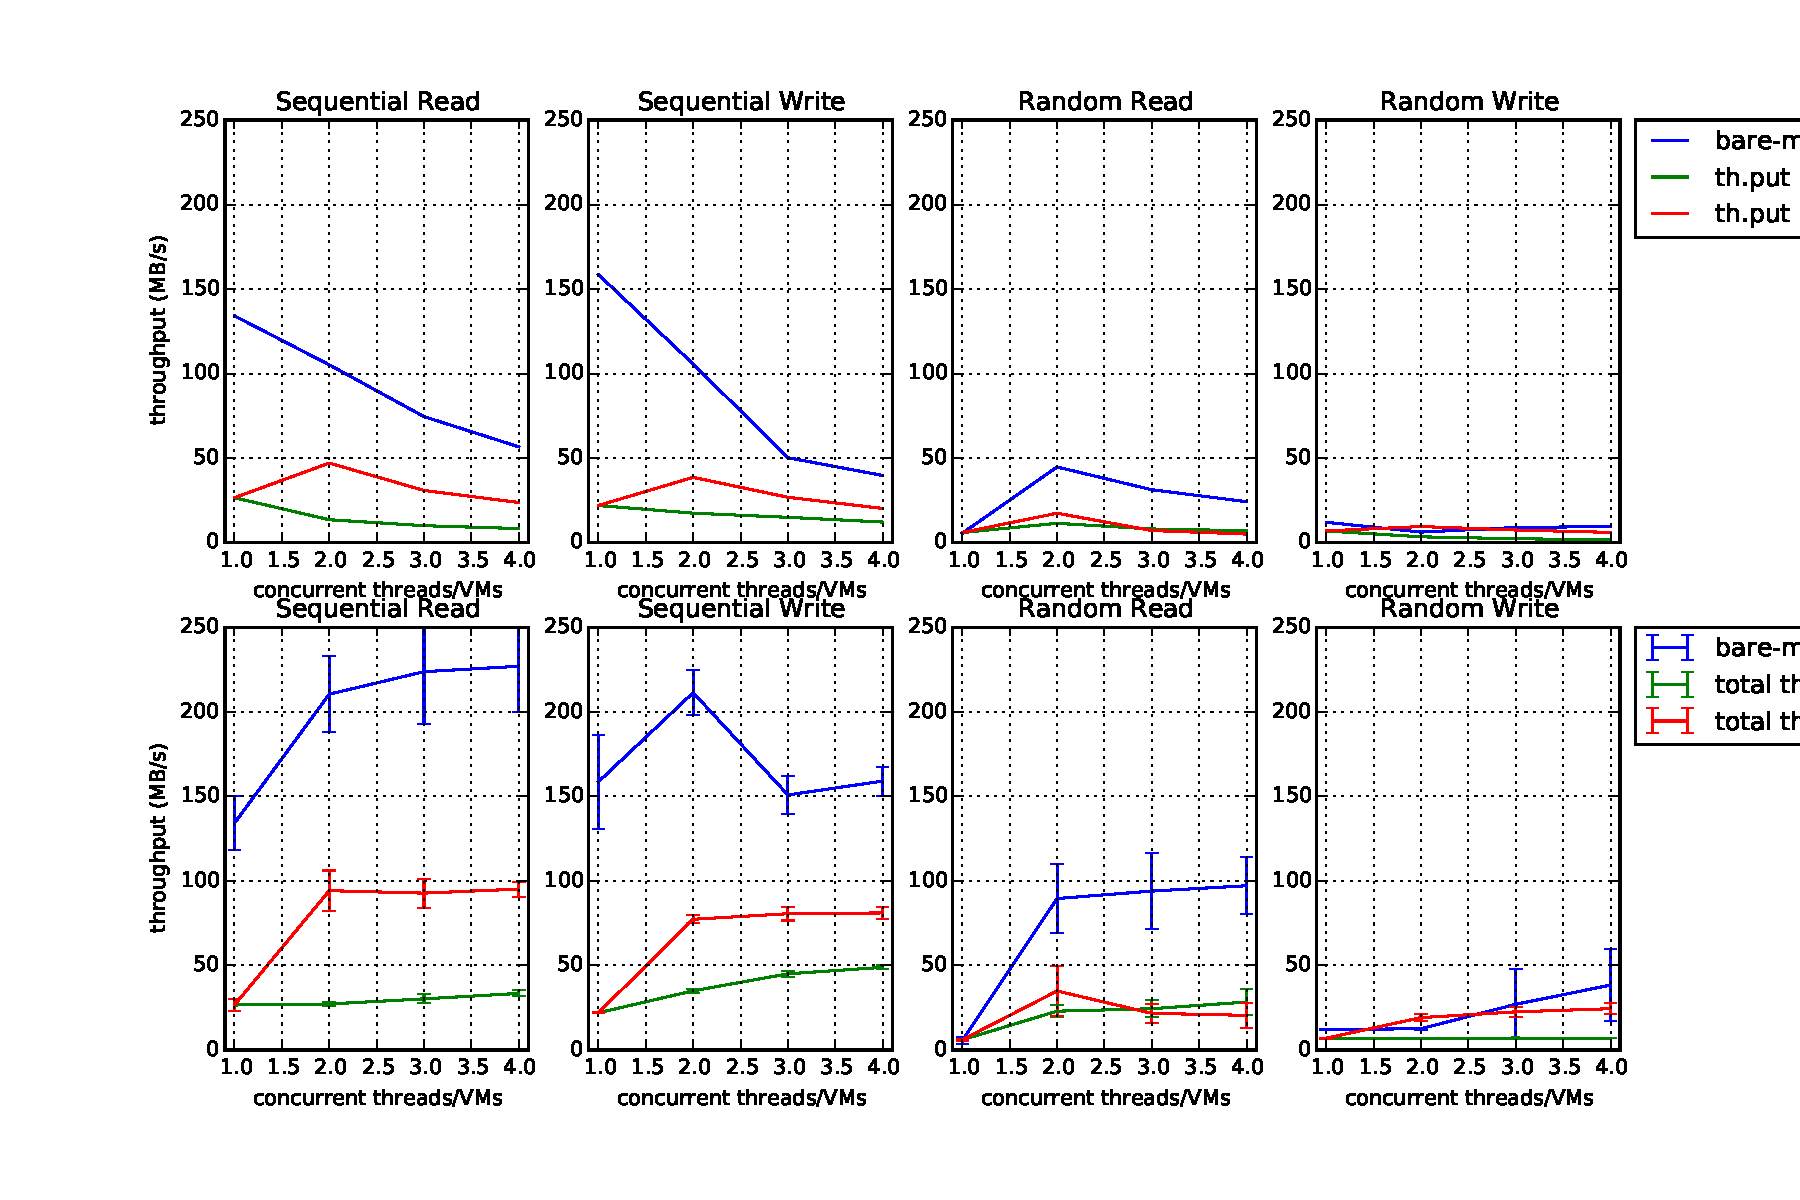
\includegraphics[scale=0.5]{throughput}
  \caption{\textit{Aggregated throughput}}
  \label{fig:throughput}
\end{figure*}

\subsubsection{Jain Fairness Index}

\begin{figure*}[t]
  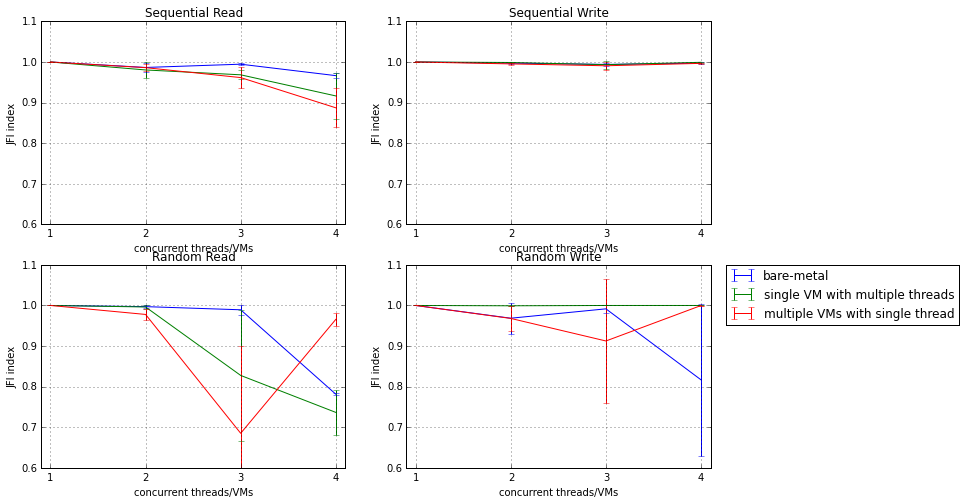
\includegraphics[scale=0.5]{JFI}
  \caption{\textit{Jain Fairness Index of the three scenarios}}
  \label{fig:jfi}
\end{figure*}

Jain Fairness Index (JFI) has a range from 0 to 1 which indicates the level of fairness between concurrent threads. If the threads receive equal partition of bandwidth, we would achieve index of 1. If only k of n flows receive equal bandwidth (and others get none), index is k/n. In the worst case, JFI has the index of 0. We plot some figures of JFI for the three scenarios with confident interval of 95\%. The figures show that threads have very equal throughput except the case of Random Read and Random Write. We notice the reader that the figures show value of JFI from 0.6 to 1.1 for a clear view on the JFI of the system. We observe from the data that in Random Read and Random Write test, JFI is low because one of thread receives very high throughput but others receive low (need to verify with different system and different test)

\subsubsection{CPU vs. Disk utilization}

\begin{figure*}[t]
  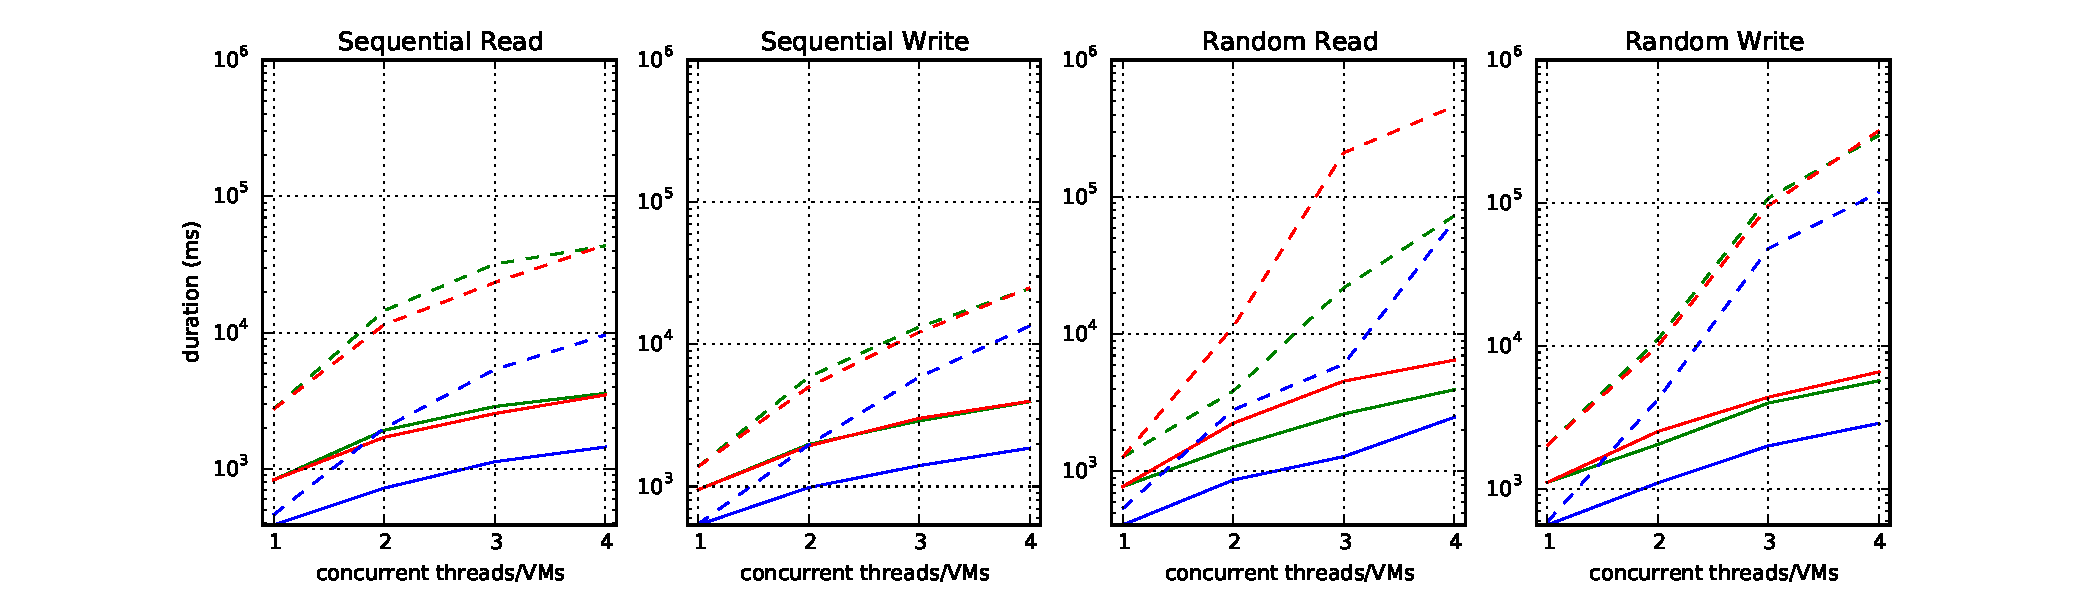
\includegraphics[scale=0.5]{CPUutilisation}
  \caption{\textit{CPU utilisation}}
  \label{fig:CPUutilisation}
\end{figure*}

The figures above represent the aggregated time for all threads to finish and the aggregated actual time that the thread are using the CPU. Because the amount of transfered data was multiplied proportional to the number of threads/VMs joining the test, so we cannot see clearly the overhead between the three scenarios. The distance between the solid line and the dash line represent the amout of useless time that the thread has to wait to finish its reading/writing. With this idea in mind, in later tests, we will use the same amount of transfered data to best present the overhead in terms of CPU utilization and CPU waiting time. The idea to use fixed data size is to see the increasing overhead when parallelism level increases.

The figures suggest that for the same amount of data, the threads inside VMs occupied the CPU more time than the bare-metal to accomplish the tasks. There is not much different between the two virtualized scenarios: Single VM with multiple threads and multiple VM with single thread. CPU spending time is a very important metric since it represent how well the process use the allocated CPU slot. For the same amount of work unit, threads inside VM spend double the time that the same ones use inside the bare-metal environment.

In bare-metal environment, the common thought is that sequential write is always slower than sequential read. But in the case of virtualized environment, we can see that sequential write is better than sequential read. The "Sequential Write" CPU utilisation can explain for the better throughput of sequential write operator in virtualized environment: because the thread running time and CPU utilisation of sequential write is less than sequential thread so we have better throughput. (Why??? maybe need to look for the way hypervisor manage the storage)

The waiting time is increasing when there are more threads accessing disk in parallel. However, because the transfer volume is increase gradually proportional to the number of parallel threads, we can not see clearly the overhead when the number of concurrent threads increases. Later experiments should fix this and draw conclusion on the behaviors of the system when parallelism is increase. These figure also lack of the disk utilisation. When disk utilisation is the bottleneck, the thread running time and CPU spending time will also increase. In later experiment, we will extract also the disk utilisation to see how it affect on CPU spending time.

\begin{figure*}[t]
  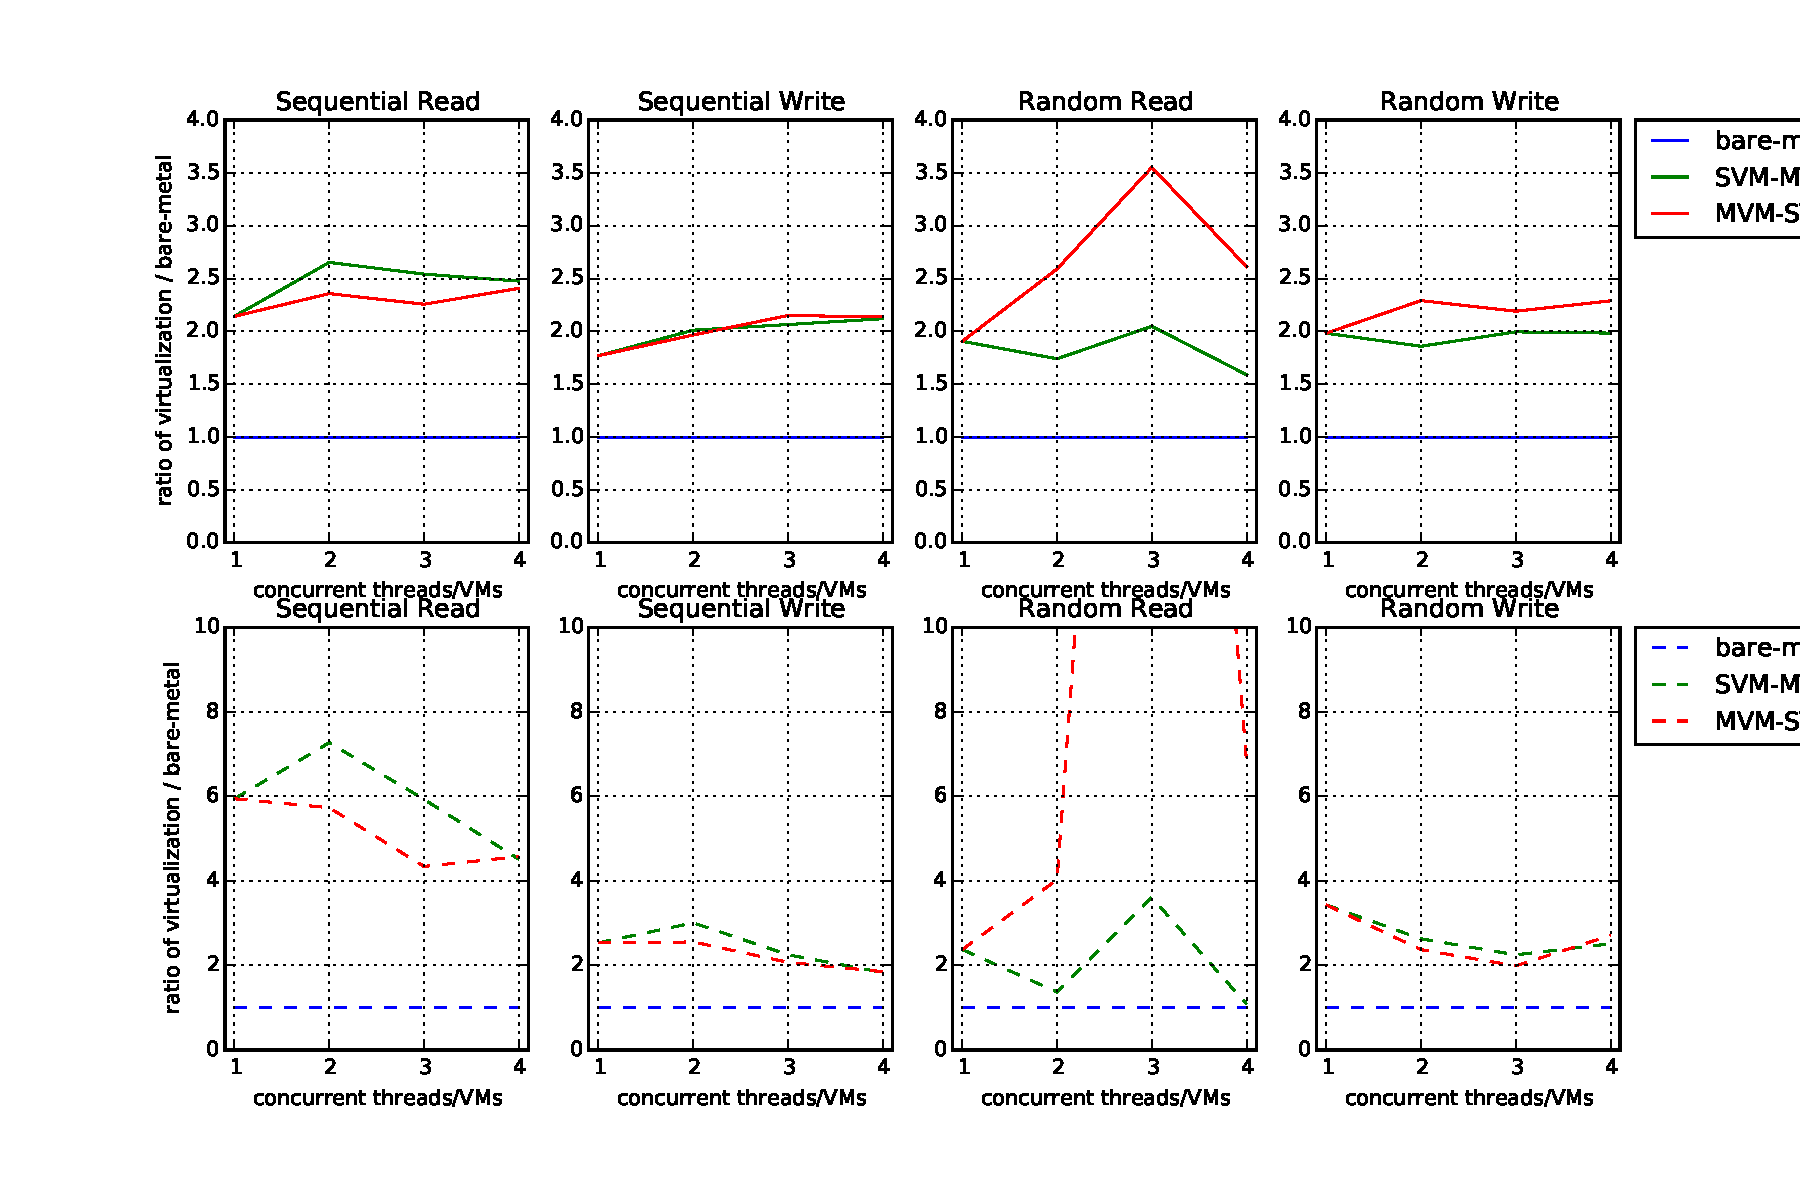
\includegraphics[scale=0.5]{nml_CPUutilisation}
  \caption{\textit{CPU utilisation after normalisation}}
  \label{fig:nml_CPUutilisation}
\end{figure*}

To illustrate the overhead in CPU spending time and Thread Running Time incurred by the virtualization, we also plot the normalisation of the CPU Spending Time and Thread Running Time figure using bare-metal data as baseline for comparison. The figures show that for the same amount of transfered data, VMs spend double the time using the CPU. They also spend more time waiting for CPU slot, about 2 to 6 times in comparing to the bare-metal. One of the reason may also due to the bottleneck at the hard disk. This one can be verified by comparing the disk utilisation of the bare-metal and the virtualized scenarios.

%%%%%%%%%%%%%%%%%%%%%%%%%%%%%%%%%%%%%%%%%%%%%%%%%%%%%%%%%%%%%%%%%%%%%





%%%%%%%%%%%%%%%%%%%%%%%%%%%%%%%%%%%%%%%%%%%%%%%%%%%%%%%%%%%%%%%%%%%%%
\section{Conclusion}
%%%%%%%%%%%%%%%%%%%%%%%%%%%%%%%%%%%%%%%%%%%%%%%%%%%%%%%%%%%%%%%%%%%%%



%%%%%%%%%%%%
% THIS PART IS FOR THE REFERENCE SECTION
%%%%%%%%%%%%
% \balance
% \bibliographystyle{abbrv}
% \bibliography{ref}

\end{document}
